\documentclass[12pt]{article}
\usepackage[english]{babel}
\usepackage[utf8]{inputenc}

%% Pointer to 'default' preamble
% pacakages and definitions

\usepackage{geometry}
\geometry{
	letterpaper, 
	portrait, 
	top=.75in,
	left=.8in,
	right=.75in,
	bottom=.5in		} 	% Page Margins
	
%% additional packages for nice things
\usepackage{amsmath} 	% for most math
\usepackage{commath} 	% for abs
\usepackage{lastpage}	% for page count
\usepackage{amssymb} 	% for therefore
\usepackage{graphicx} 	% for image handling
\usepackage{wrapfig} 	% wrap figures
\usepackage[none]{hyphenat} % for no hyphenations
\usepackage{array} 		% for >{} column characterisctis
\usepackage{physics} 	% for easier derivative \dv....
\usepackage{tikz} 		% for graphic@!
\usepackage{circuitikz} % for circuits!
\usetikzlibrary{arrows.meta} % for loads
\usepackage[thicklines]{cancel}	% for cancels
\usepackage{xcolor}		% for color cancels
\usepackage[per-mode=fraction]{siunitx} % for si units and num
\sisetup{group-separator = {,}, group-minimum-digits = 3} % additional si unit table functionality

\usepackage{fancyhdr} 	% for header
\usepackage{comment}	% for ability to comment out large sections
\usepackage{multicol}	% for multiple columns using multicols
\usepackage[framed,numbered]{matlab-prettifier} % matlab sytle listing
\usepackage{marvosym} 	% for boltsymbol lightning
\usepackage{pdflscape} 	% for various landscape pages in portrait docs.
%\usepackage{float}
\usepackage{fancyvrb}	% for Verbatim (a tab respecting verbatim)
\usepackage{enumitem}	% for [resume] functionality of enumerate
\usepackage{spreadtab} 	% for using formulas in tables}
\usepackage{numprint}	% for number format in spread tab
\usepackage{subcaption} % for subfigures with captions
\usepackage[normalem]{ulem} % for strike through sout

% for row colors in tables....
\usepackage{color, colortbl}
\definecolor{G1}{gray}{0.9}
\definecolor{G2}{rgb}{1,0.88,1}%{gray}{0.6}
\definecolor{G3}{rgb}{0.88,1,1}

% For table formatting
\usepackage{booktabs}
\renewcommand{\arraystretch}{1.2}
\usepackage{floatrow}
\floatsetup[table]{capposition=top} % put table captions on top of tables

% Caption formating footnotesize ~ 10 pt in a 12 pt document
\usepackage[font={small}]{caption}

%% package config 
\sisetup{output-exponent-marker=\ensuremath{\mathrm{E}}} % for engineer E
\renewcommand{\CancelColor}{\color{red}}	% for color cancels
\lstset{aboveskip=2pt,belowskip=2pt} % for more compact table
%\arraycolsep=1.4pt\def
\setlength{\parindent}{0cm} % Remove indentation from paragraphs
\setlength{\columnsep}{0.5cm}
\lstset{
	style      = Matlab-editor,
	basicstyle = \ttfamily\footnotesize, % if you want to use Courier - not really used?
}
\renewcommand*{\pd}[3][]{\ensuremath{\dfrac{\partial^{#1} #2}{\partial #3}}} % for larger pd fracs
\renewcommand{\real}[1]{\mathbb{R}\left\{ #1 \right\}}	% for REAL symbol
\newcommand{\imag}[1]{\mathbb{I}\left\{ #1 \right\}}	% for IMAG symbol
\definecolor{m}{rgb}{1,0,1}	% for MATLAB matching magenta
	
%% custom macros
\newcommand\numberthis{\addtocounter{equation}{1}\tag{\theequation}} % for simple \numberthis command

\newcommand{\equal}{=} % so circuitikz can have an = in the labels
\newcolumntype{L}[1]{>{\raggedright\let\newline\\\arraybackslash\hspace{0pt}}m{#1}}
\newcolumntype{C}[1]{>{\centering\let\newline\\\arraybackslash\hspace{0pt}}m{#1}}
\newcolumntype{R}[1]{>{\raggedleft\let\newline\\\arraybackslash\hspace{0pt}}m{#1}}

%% Header
\pagestyle{fancy} % for header stuffs
\fancyhf{}
% spacing
\headheight 29 pt
\headsep 6 pt

%% Header
\rhead{Thad Haines \\ Page \thepage\ of \pageref{LastPage}}
\chead{Mini WECC \\   10 Minute AGC Recovery}
\lhead{Research \\ 08/17/20}

\usepackage[hidelinks]{hyperref} % allow links in pdf
\usepackage{setspace}
\usepackage{multicol}
\usepackage{minted}

\begin{document}
\onehalfspacing
\paragraph{10 Minute AGC Recovery of Mini WECC after 435 MW Load Step} \ \\

\begin{minipage}{0.47\linewidth}
\begin{itemize}
\item Mini WECC system:
\begin{itemize}
\itemsep 0 em
\small
\item Buses: 122
\item Lines: 171
\item Loads: 88
\item Machines: 34
\item States: 623
\end{itemize}
\item Event: +435 MW load step on Bus 2\\in Area 1 at t=1.

\item Each area has identical conditional AGC that acts at t=40 and again when t=160, 280, 400, 520 (i.e. 2 minute action time).

\item ODE solver tolerances:
\subitem Relative: 1e-5
\subitem Absolute: 1e-7

\end{itemize}
\vfill
\end{minipage}\hspace{2em}% 
\begin{minipage}{0.47\linewidth}
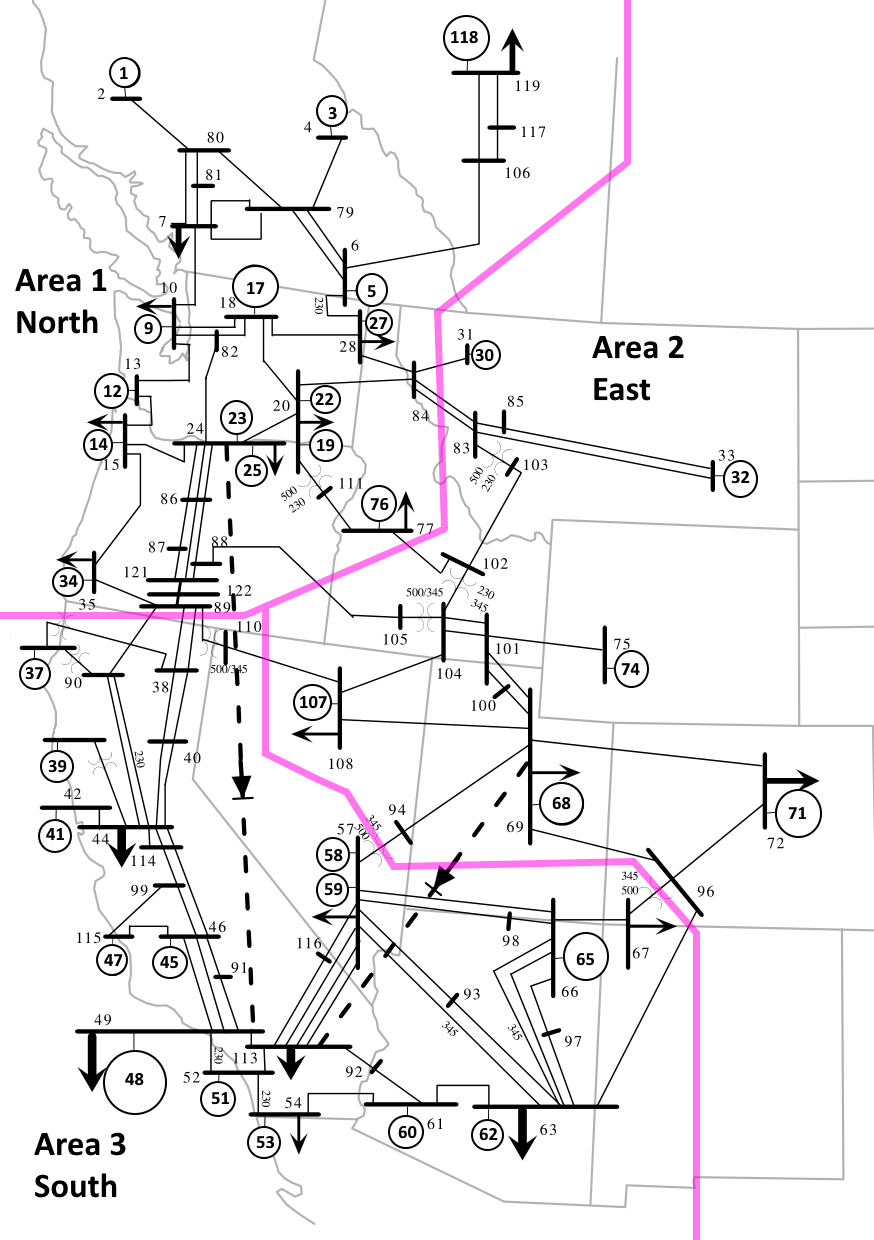
\includegraphics[width=.9\linewidth]{miniWECC_split03.png}
\end{minipage}% 

\paragraph{Result Summary:}
\begin{itemize}
\item Using the ode23/ode23t methods provided a 9 times speed up over Huen's `fixed step' method.
\item  27 times fewer steps were taken using VTS which resulted with a saved file size that was approximately 24 times smaller than the Huen's method data file.
\item VTS methods appeared to capture fast dynamics well. 
\item VTS and fixed time step results  may `drift' slightly when time steps become large. \\ Effect can be reduced via ODE solver tolerance settings or additional \verb|sw_con| time blocks.

\end{itemize}
\begin{table}[!ht]
\resizebox{\linewidth}{!}{

	\begin{tabular}{@{} L{1.75cm} 
	R{2cm} R{2cm}  R{2cm} R{1.5cm} R{0.75cm} R{1cm} R{1.5cm} R{2cm} R{2.5cm}@{}} 	
		\toprule % @ signs to remove extra L R space
		\footnotesize % this will affect the table font (makse it 10pt)
		\raggedright % for non justified table text

			&	\multicolumn{3}{c}{Step Size [seconds]}					&		&	\multicolumn{2}{c}{\shortstack{Solutions\\Per Step}}			&		&		&		\\	
		Method	&	Max	&	Min	&	Ave	&	Total Steps	&	Ave	&	Max	&	Total Slns.	&	Sim. Time [seconds]	&	File Size [bytes]	\\ \midrule	
		Huen's	&	0.0083	&	8.33E-03	&	0.0083	&	72,001	&	2	&	2	&	144,002	&	483.64	&	778,259,381	\\	
		ode23/ ode23t	&	8.6300	&	1.19E-06	&	0.0570	&	2,662	&	2	&	775	&	6,632	&	53.4	&	32,772,591	\\	\midrule
		$\Delta$Ratio	&	0.001	&	7,000	&	0.146	&	27.05	&	1	&	0.003	&	21.71	&	9.06	&	23.75	\\	\bottomrule

	\end{tabular}
	}%end resize box
\end{table}

\pagebreak
\paragraph{Step Size and Solution Count Data} \ \\
Time blocks were created at: [0:1], [1:40], and [40:600].
Many solutions were executed at beginning of each blocks due to ODE solver method \emph{possibly} creating a Jacobian.\\

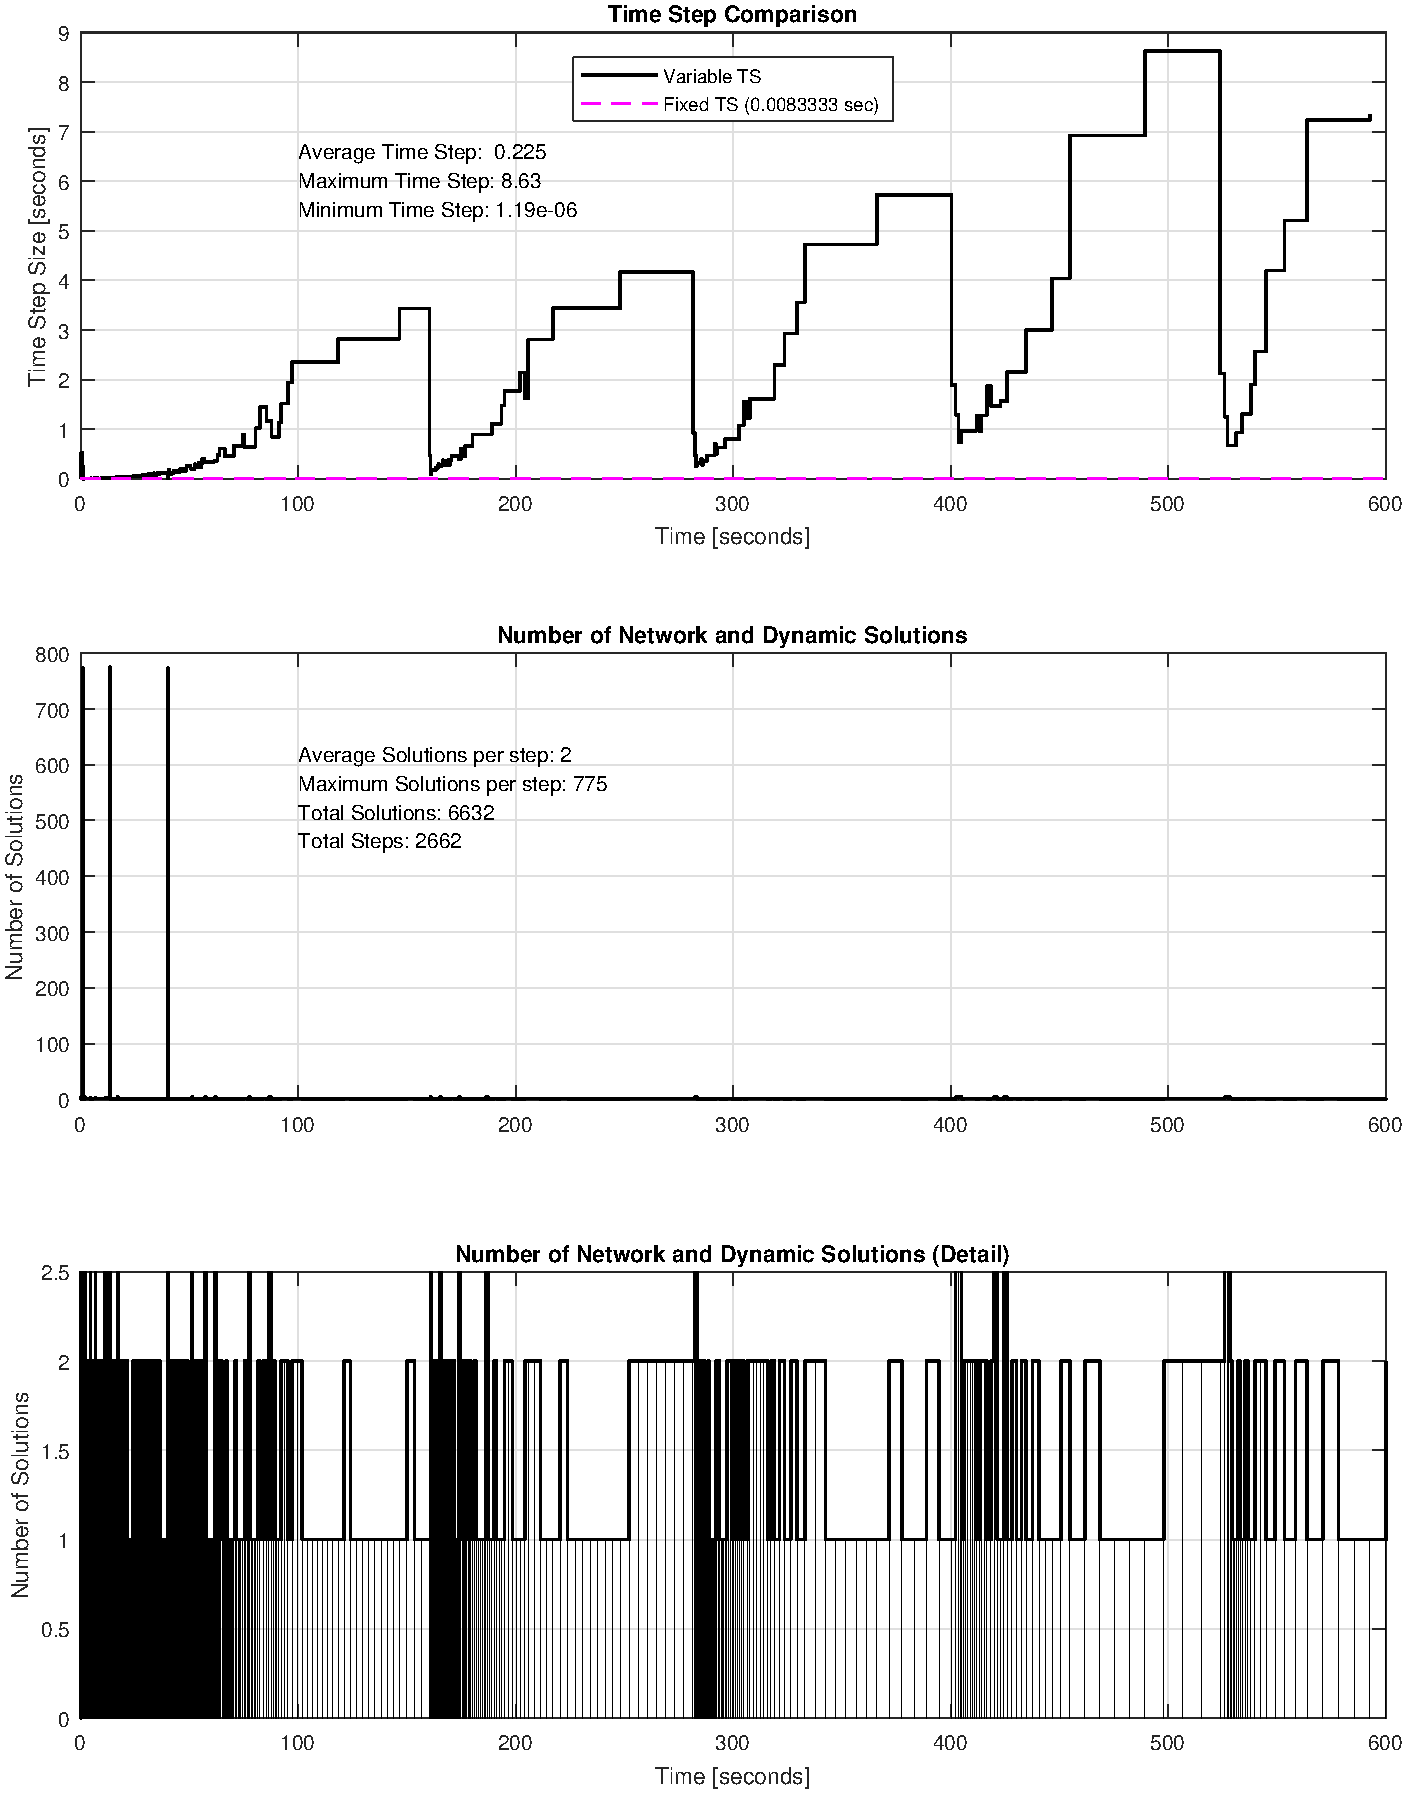
\includegraphics[width=.97\linewidth]{MWstepComp}

\pagebreak
\paragraph{Select Comparisons: t = 0:600 (full simulation)} \ \\
Simulation had a lot of time where not many fast dynamic changes were taking place. \\


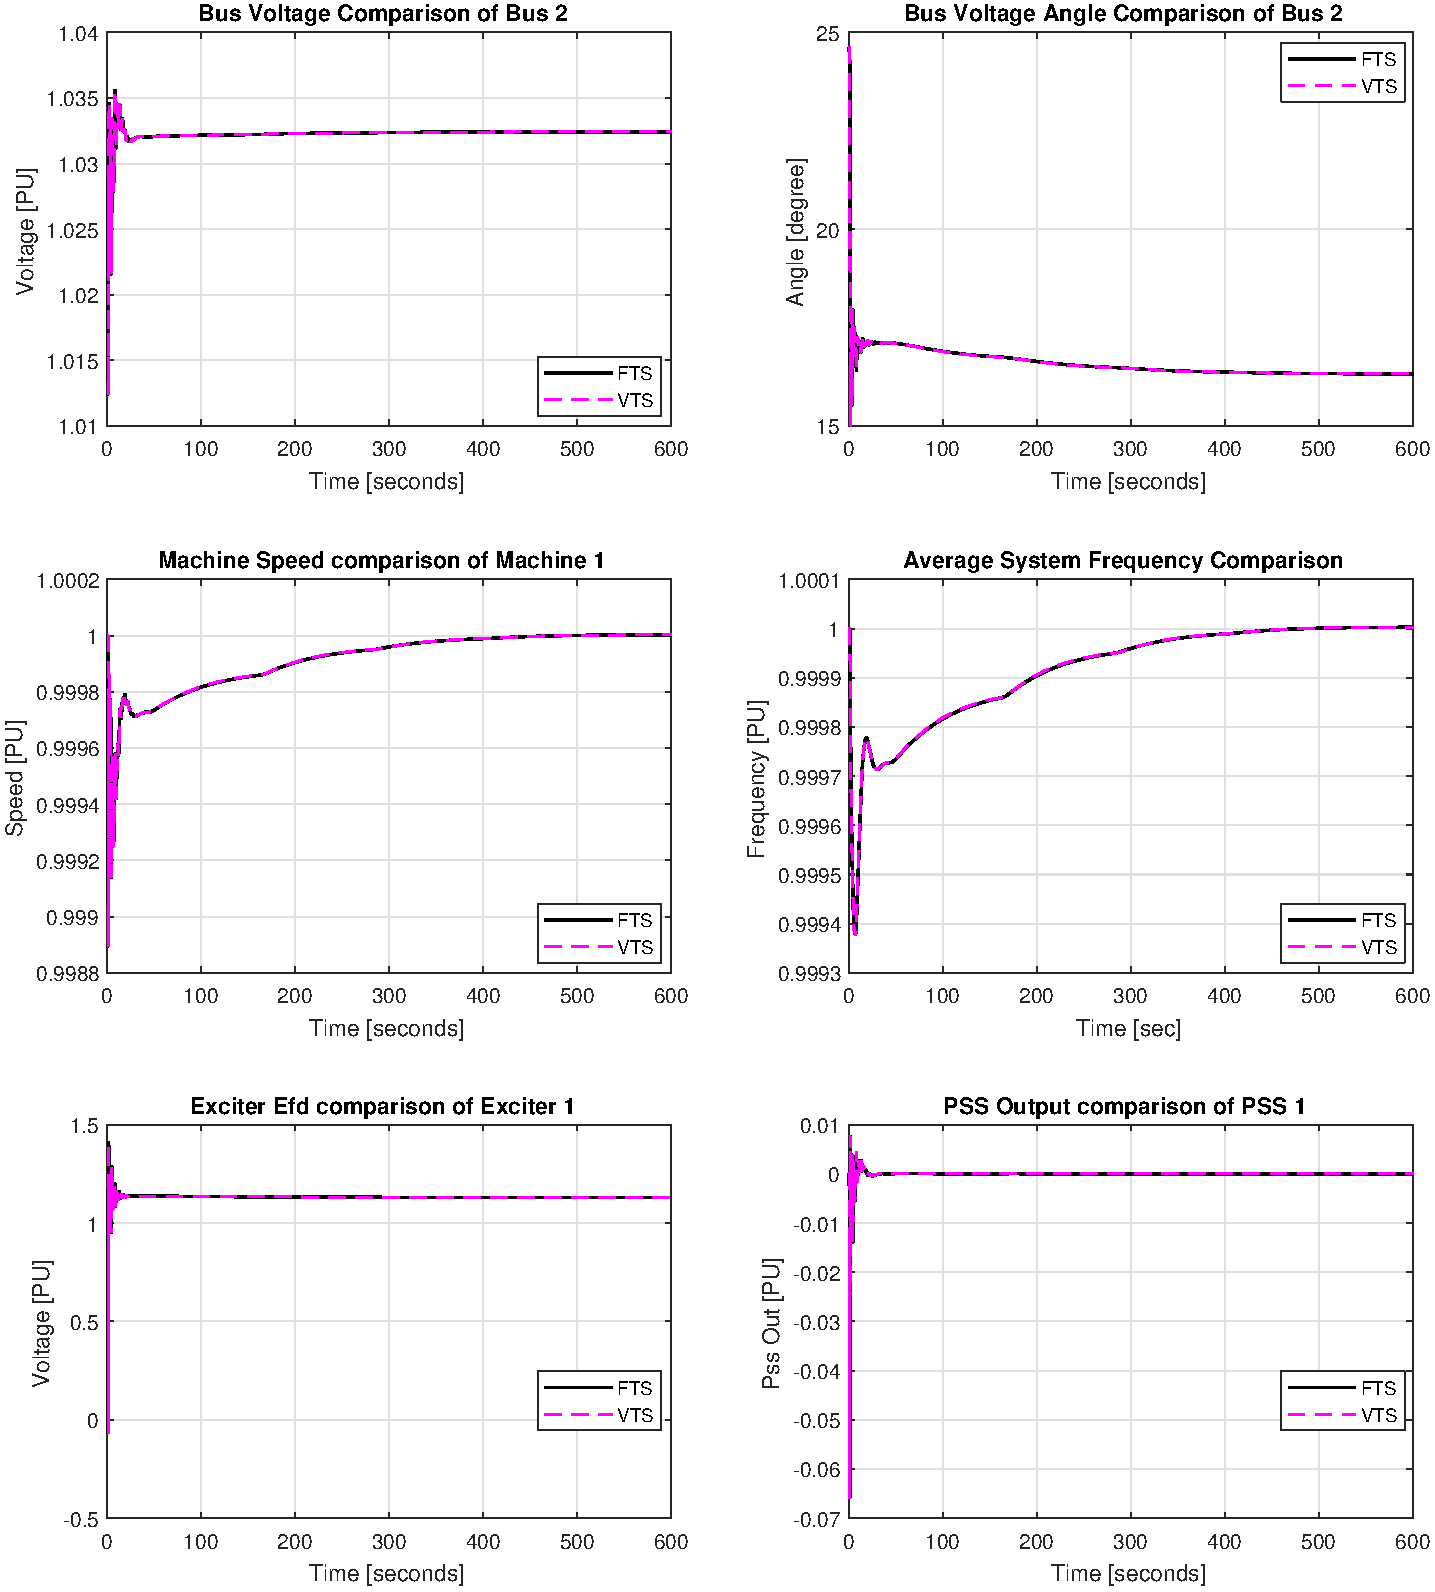
\includegraphics[width=\linewidth]{MWdetailFull}

\pagebreak
\paragraph{Select Comparisons: t = 0:10} \ \\
Initial transients were captured well.\\

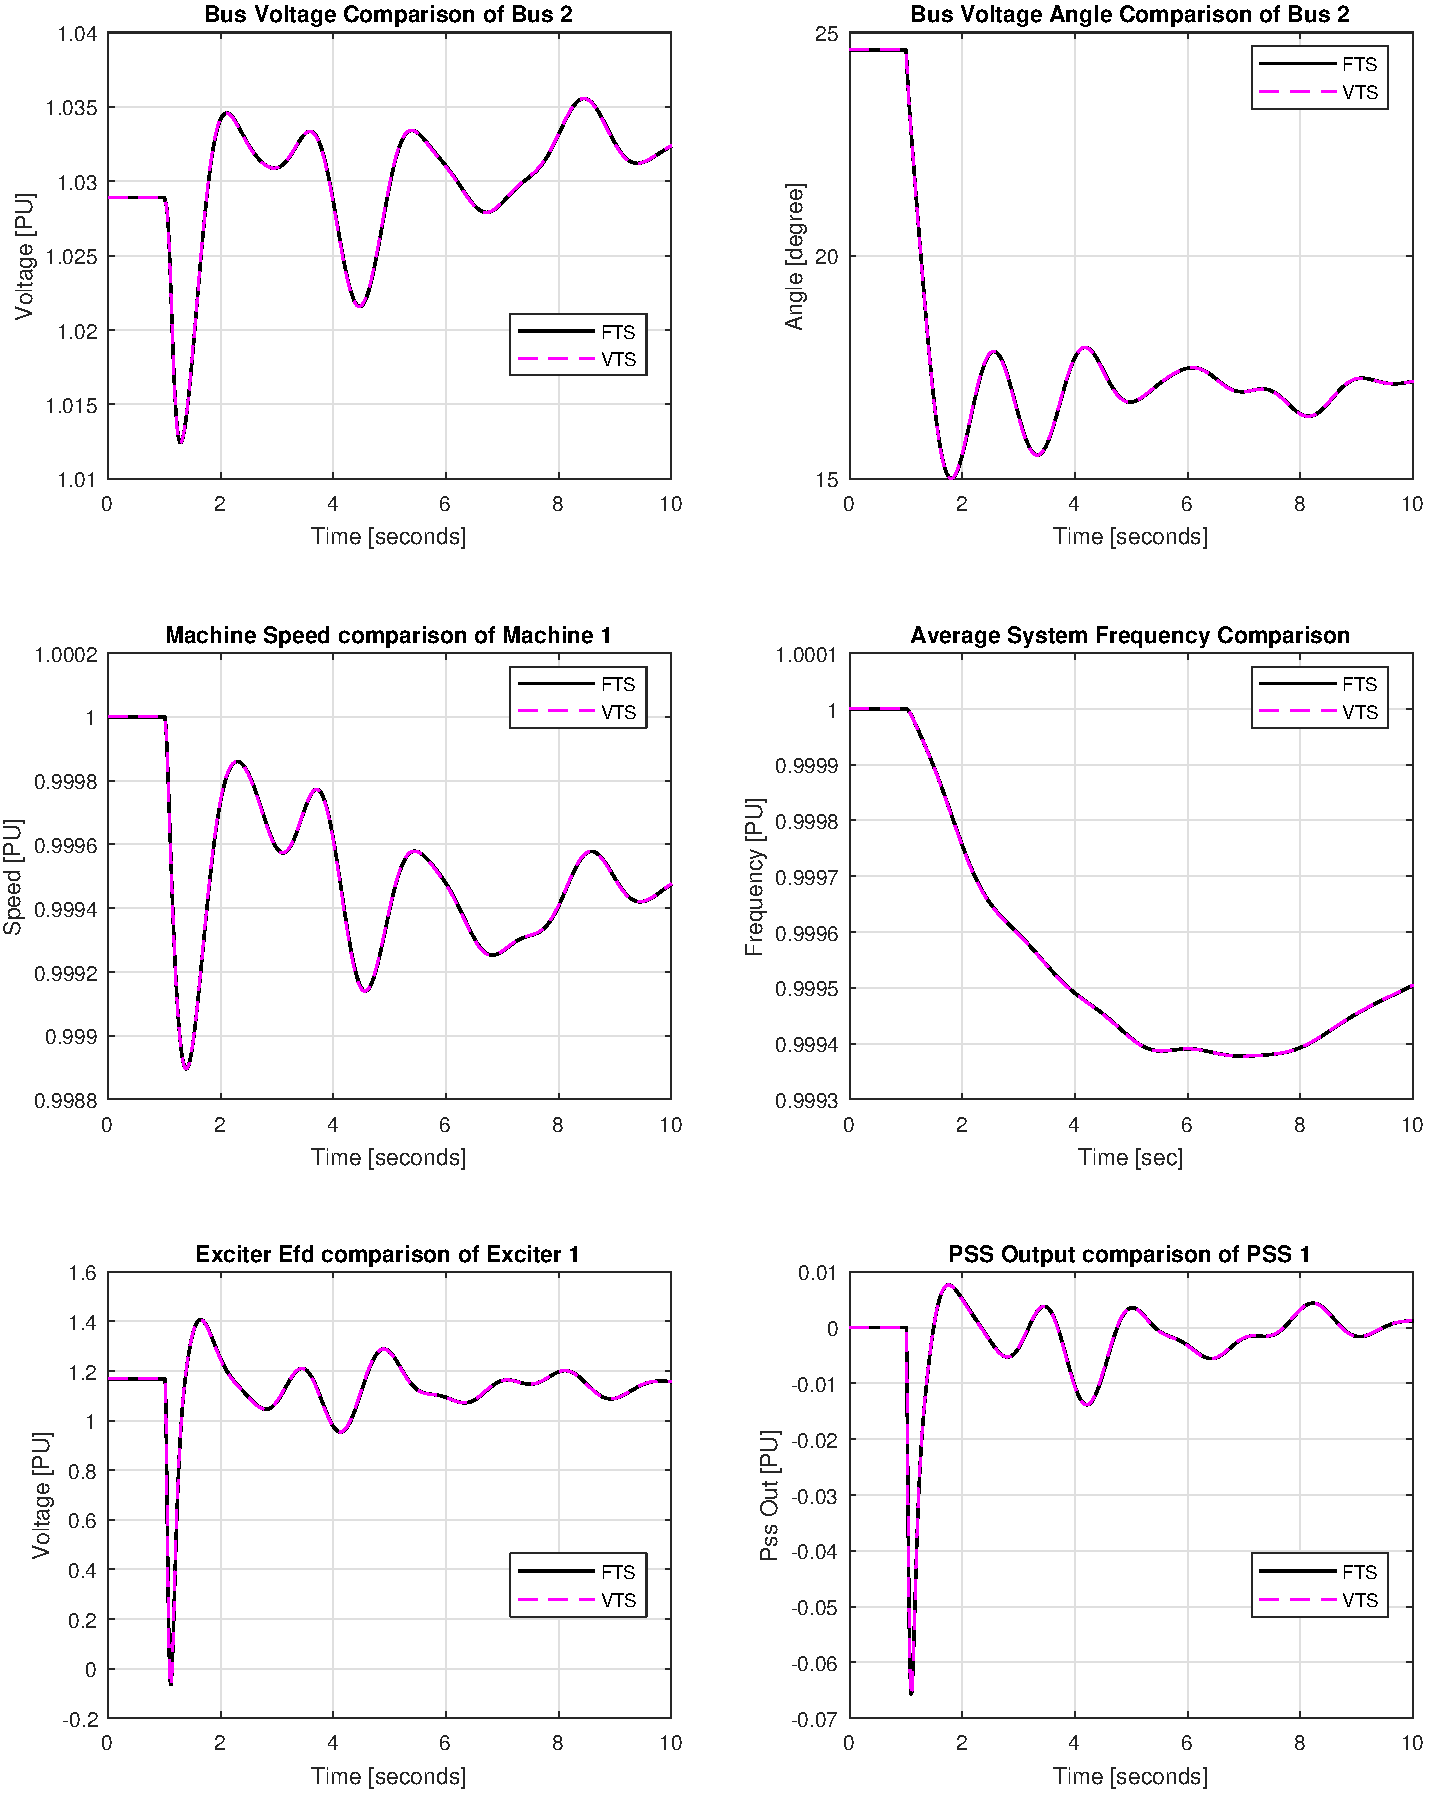
\includegraphics[width=\linewidth]{MWdetailComp0}

\pagebreak
\paragraph{Select Comparisons: t = 0:40} \ \\
Simulation methods continued to match as system stabilized.\\

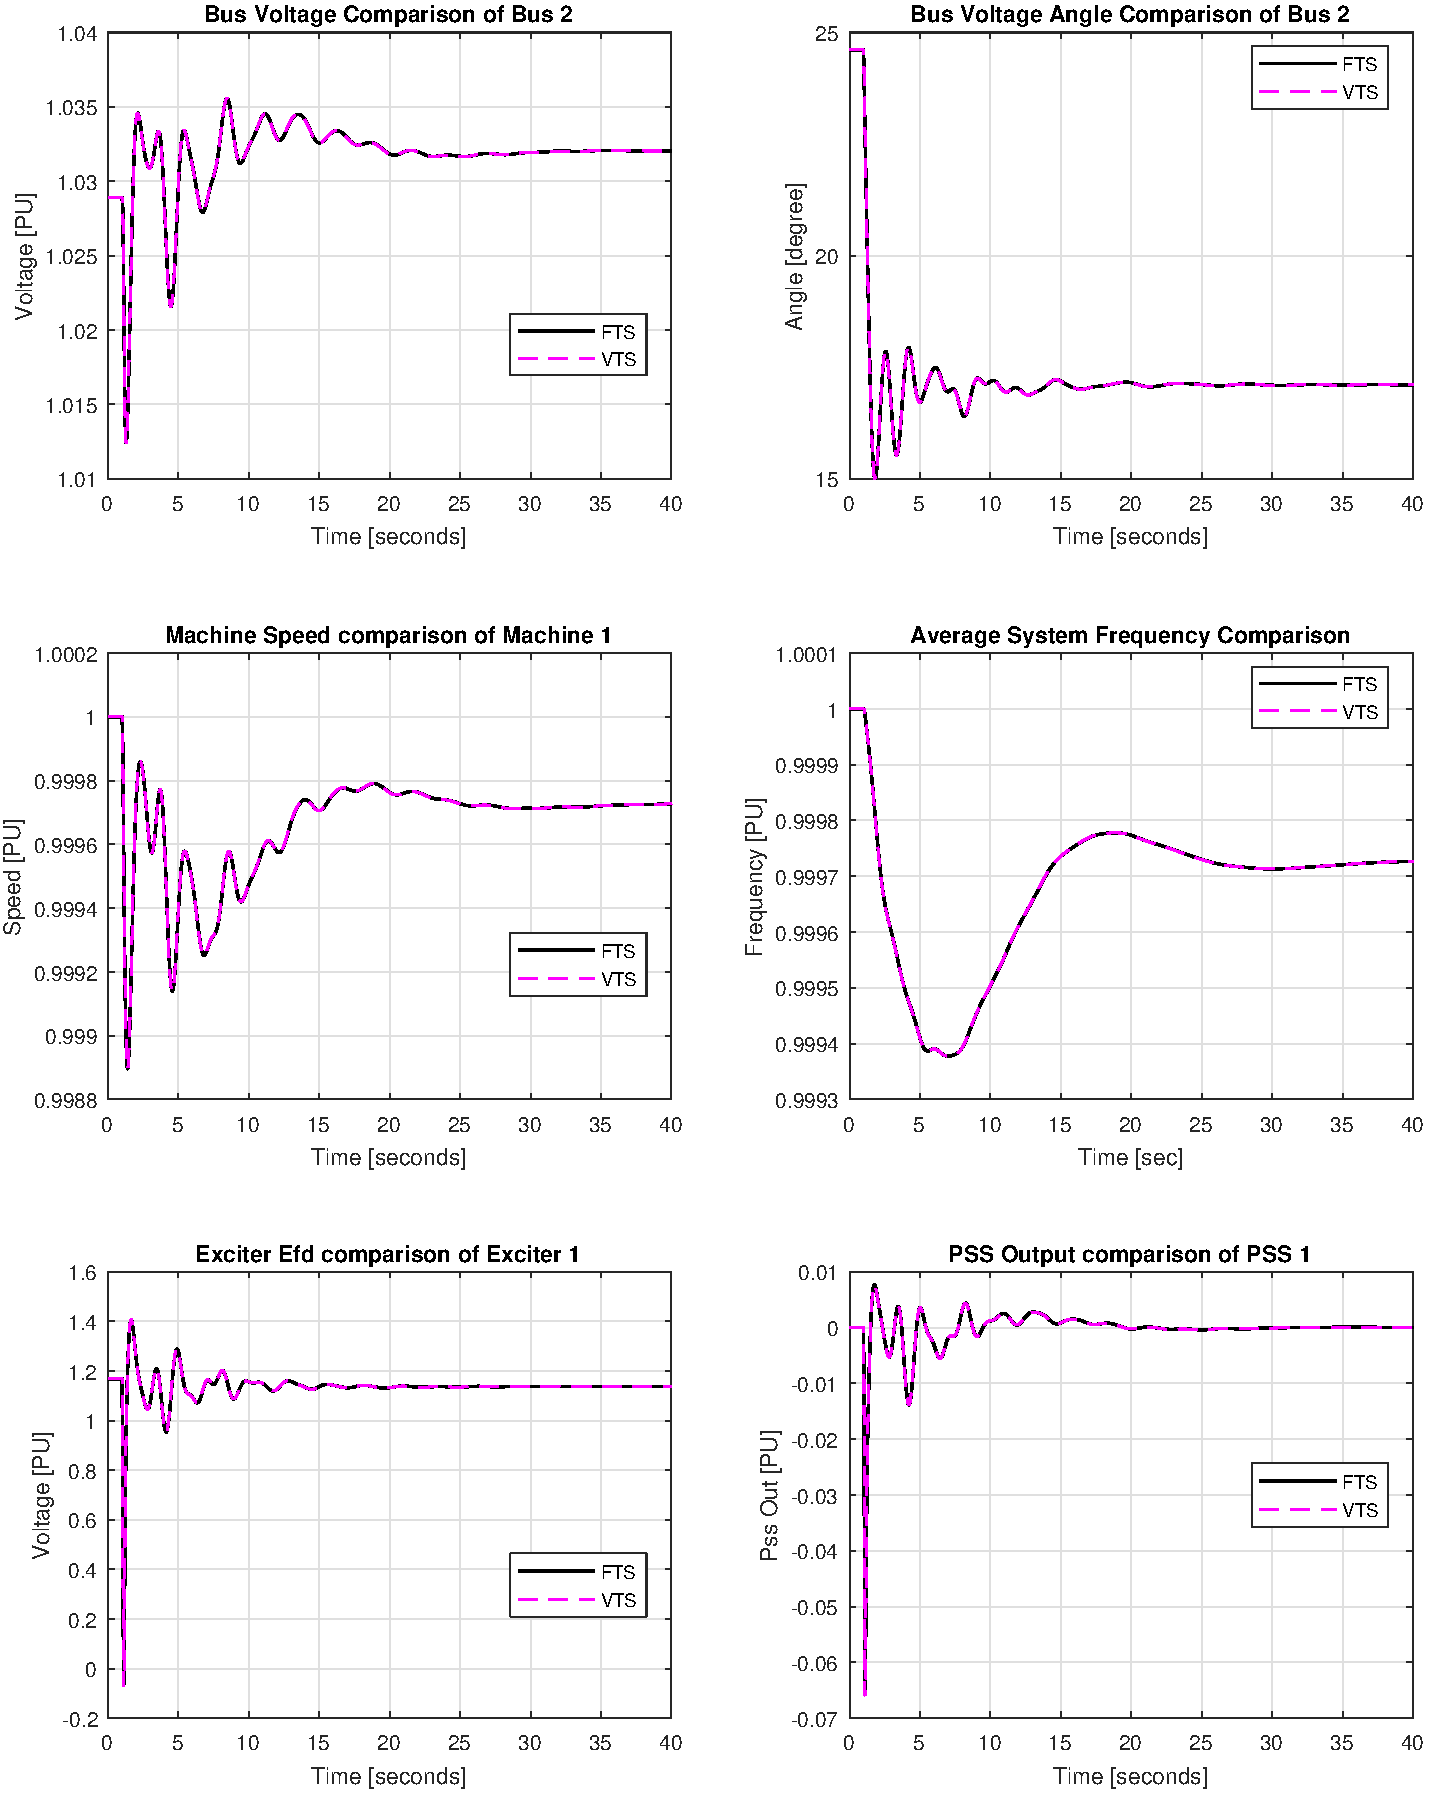
\includegraphics[width=\linewidth]{MWdetailComp1}


\pagebreak
\paragraph{Select Comparisons: t = 260:360 (Result `Drift' - Scale should be noted)} \ \\
As individual time blocks were not created for each AGC action, dispatches may not be synchronized between simulations and add to state drift. \\

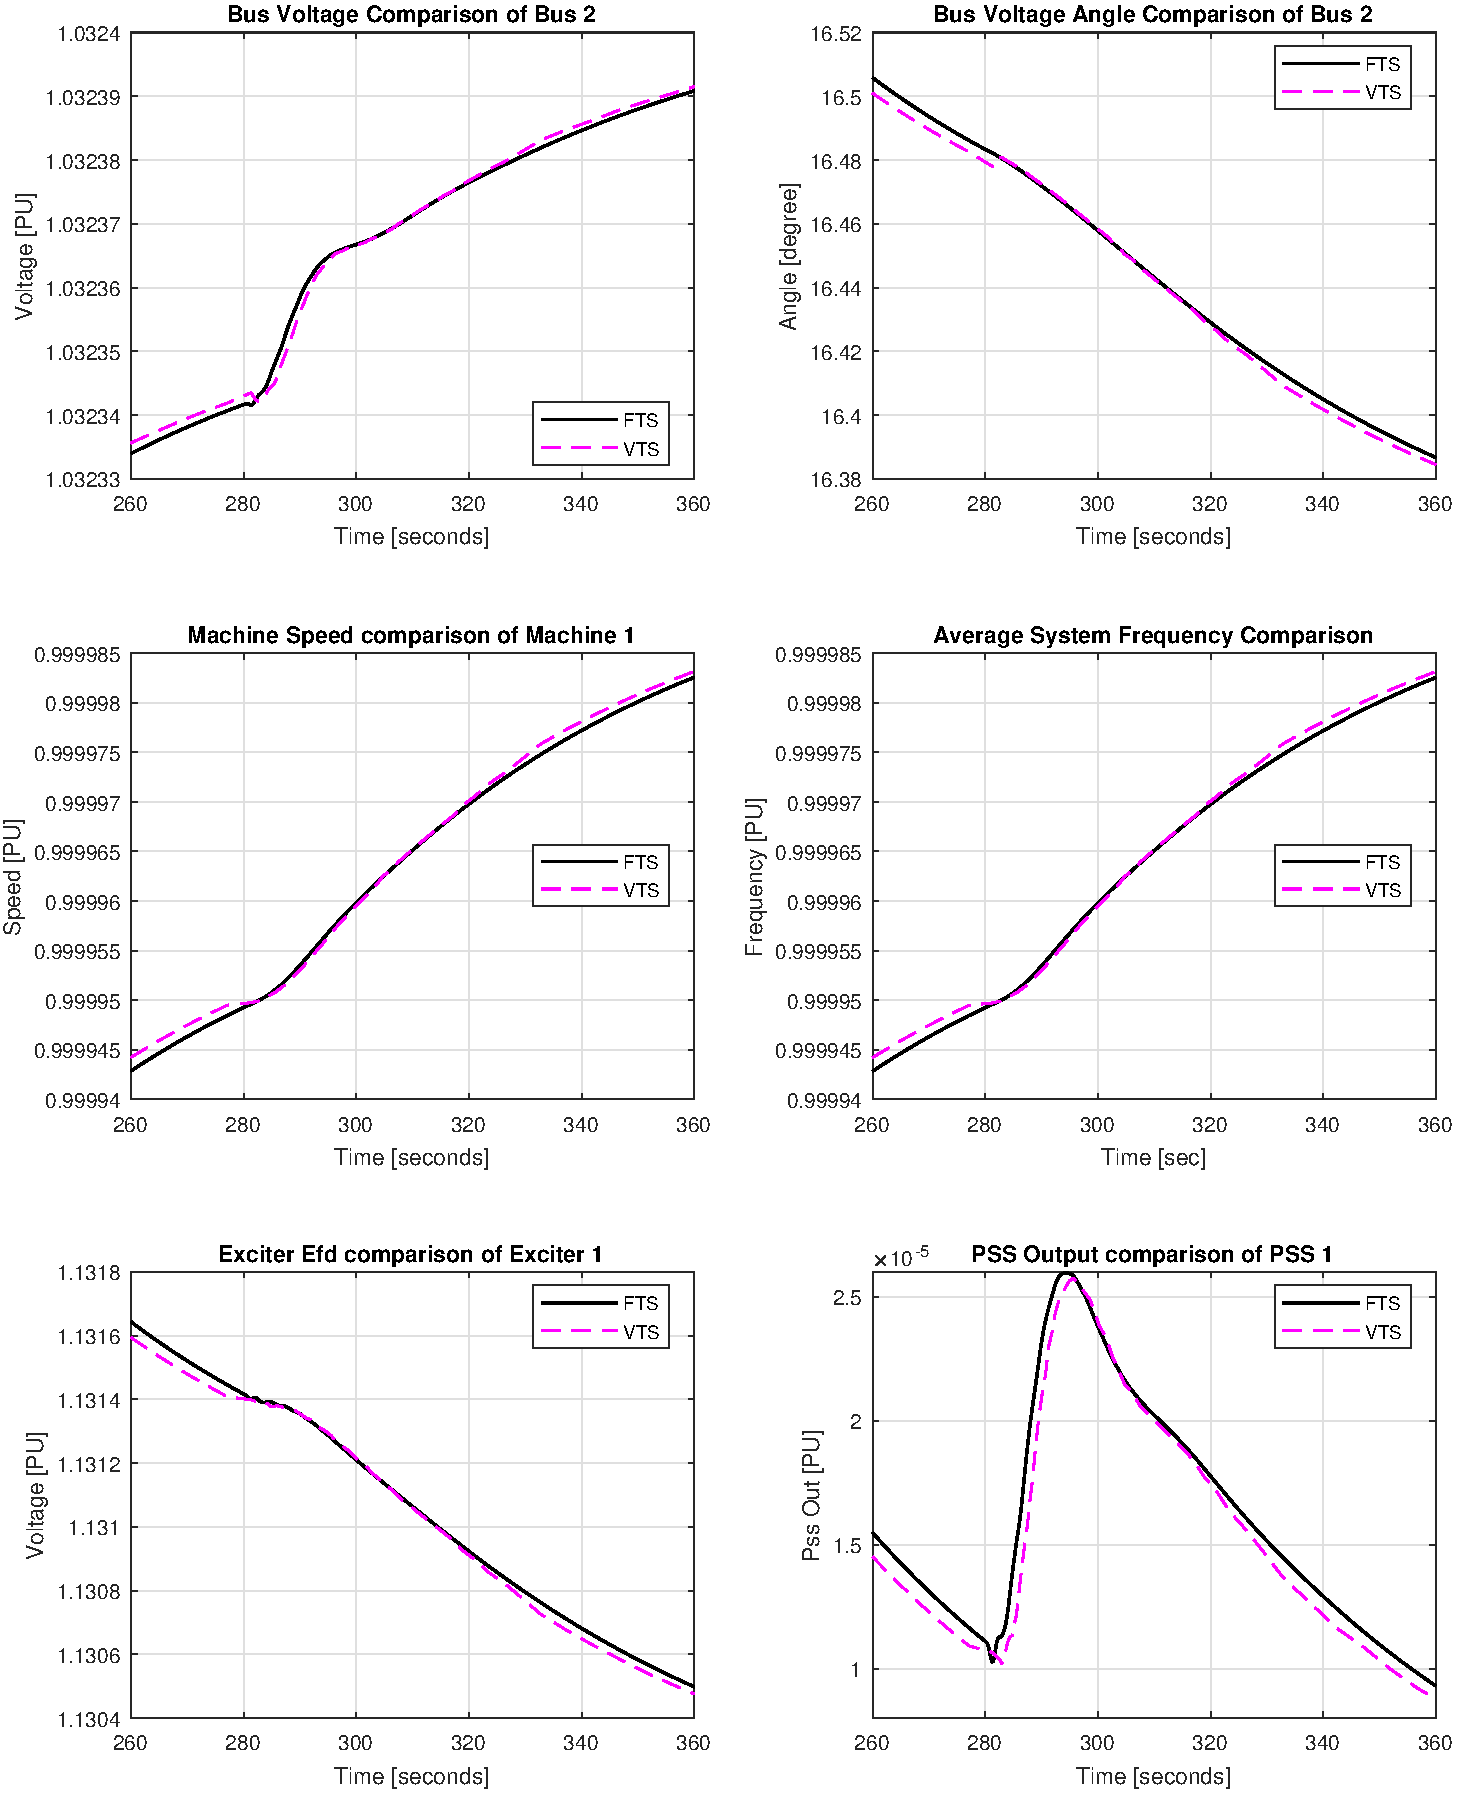
\includegraphics[width=\linewidth]{MWdetailComp2}
\pagebreak
\paragraph{AGC Settings} \ \\
\vspace{-2em}

\begin{minted}[
		frame=lines,
		framesep=2mm,
		baselinestretch=1.2,
		bgcolor=gray!13,
		fontsize=\footnotesize,
		linenos,
		breaklines
		]{MATLAB}
%{ 
Each agc(x) has following fields:
    area        - Area number / controlled area
    startTime   - Time of first AGC signal to send
    actionTime  - Interval of time between all following AGC signals
    gain        - Gain of output ACE signal
    Btype       - Fixed frequency bias type (abs, percent of max capacity...)
        0 - absolute - Input B value is set as Frequency bias (positive MW/0.1Hz)
        1 - percent of max area capacity
    B           - Fixed frequency bias Value
    Kbv         - Varaible frequency bias gain used to gain B as B(1+kBv*abs(delta_w))
    condAce     - Conditional ACE flag
        0 - Conditional ACE not considered
        1 - ace2dist updated only if sign matches delta_w (i.e. in area event)

    (PI Filter Values)
    Kp          - Proportional gain
    a           - ratio between integral and proportional gain (placement of zero)
    ctrlGen_con - col 1 = generator bus, 
                  col 2 = participation factor, 
                  col 3 = low pass filter time constant [seconds]
%}
agc(1).area = 1;
agc(1).startTime = 40;
agc(1).actionTime = 120;
agc(1).gain = 1; % gain of output signal
agc(1).Btype = 1; % per max area capacity
agc(1).B = 1;
agc(1).Kbv = 0; % no variable bias
agc(1).condAce = 1; % conditional ACE
agc(1).Kp = 0.015;
agc(1).a = 0.0001;
agc(1).ctrlGen_con = [ 23, 1.0, 60 ];

agc(2) = agc(1); % duplicate most settings from AGC 1 to AGC 2
agc(2).area = 2;
agc(2).ctrlGen_con = [ 32, 1.0, 60 ];

agc(3)=agc(1); % duplicate most settings from AGC 1 to AGC 3
agc(3).area = 3;
agc(3).ctrlGen_con = [...
    45, 0.75, 60;
    53, 0.25, 60;
    ];
\end{minted}
\end{document}
